\section*{Assignment 07: Inequality and Responsibility}
\addcontentsline{toc}{section}{Assignment 07: Inequality and Responsibility}

I begin by mapping who falls through the cracks on SkillSync. Resource-light NGOs lack cash and staff to babysit another dashboard and fear hidden fees or data obligations of the kind \citet{Srnicek2017} critiques. Humanities and design faculties also risk being sidelined because their success metrics differ from the business school crowd, echoing \citet{Choudary2016}'s point that governance must match each segment’s value logic.

To make life easier for NGOs I propose a ``lean onboarding kit'': a ready-made data sheet, templated event briefs, and an access programme where we pair them with students during the first weeks. In the VirtuAI case the social onboarding layer was crucial for getting nonprofits involved precisely because their resources were thin \citep{Gunasilan2024}. Practically that means a lightweight flow with clear budget caps and auto-generated reports so organisations skip building measurement tools from scratch.

When I look at faculties, the design move is to let them shape their own micro-communities. We can spin up ``faculty sandboxes'' where humanities define alternative engagement metrics while economists stick with classic growth curves. That mirrors \citet{Reillier2017}'s advice on modular governance layers that avoid locking communities into a single logic. We should also stay open to certain faculties experimenting with analogue events that can be documented via simple upload forms rather than mandatory livestreaming.

On the policy side I sketch three straightforward rules. First a fairness clause committing us to track resource spend per organisation and offer fee waivers if volunteer hours exceed a certain threshold. That dovetails with \citet{ShapiroVarian1999}, who note that subsidising the weaker side can accelerate network effects. Second an inclusion policy granting every faculty a seat on a data-and-ethics council so we avoid governance bias---something \citet{Zuboff2019} flags as a classic trap in surveillance capitalism. Third a recurring impact audit inspired by the DineTogether case, where every quarter we review whether features inadvertently favour resource-rich actors \citep{Rennella2023}.

As an overarching design principle I stick with ``progressive engagement'': the more resources an actor has, the more advanced tools we unlock, while the baseline experience stays simple and free. It operationalises both the theoretical demand for balanced network effects and the pragmatic lessons from our cases. NGOs with minimal budgets and faculties with divergent success criteria can still join without feeling overwhelmed, while ambitious partners still see a path to deeper collaboration.

Figure~\ref{fig:chat-system} captures the messaging system that underpins this fairness work. The chat interface handles micro-coaching, inclusion triage, and governance updates in plain language. Students can flag ``access support needed'' for quick moderator response, NGOs can request translation help, and templated replies reference our fairness clause so tone stays consistent when moderators rotate.

\begin{figure}[h]
  \centering
  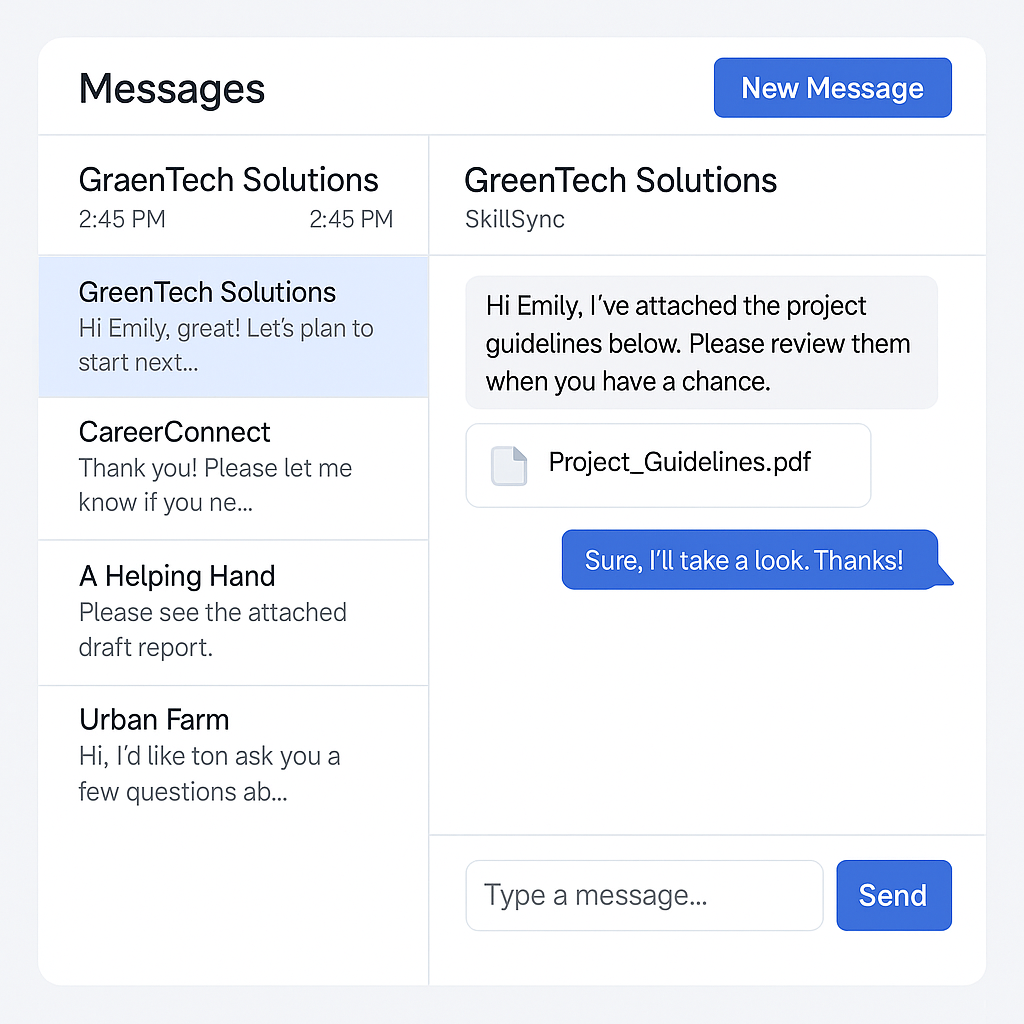
\includegraphics[width=0.85\linewidth]{meddelelsessystem-chatfunktion.png}
  \caption{Messaging workspace (`meddelelsessystem-chatfunktion.png`) used for inclusive support and moderation.}
  \label{fig:chat-system}
\end{figure}

I also introduced a ``mutual aid'' feature where resource-rich partners can volunteer surplus capacity (design time, translation, access to datasets) to NGOs struggling with bandwidth. The chat system coordinates those offers, ensuring credits get logged and recognition flows back to contributors so inequality does not harden as we scale.
